\section{Tutorial}\label{Tutorial}

The tutorial describes few main cases of the arbitrary user, neural network engineer and contributor user. The use cases will be described in UML  Activity Diagram. The details will be skipped, only the main function will be described.  

\subsection{Using Network and Model Repositories}\label{Using Network and Model Repositories}

\begin{figure}[htbp]
\begin{center}
  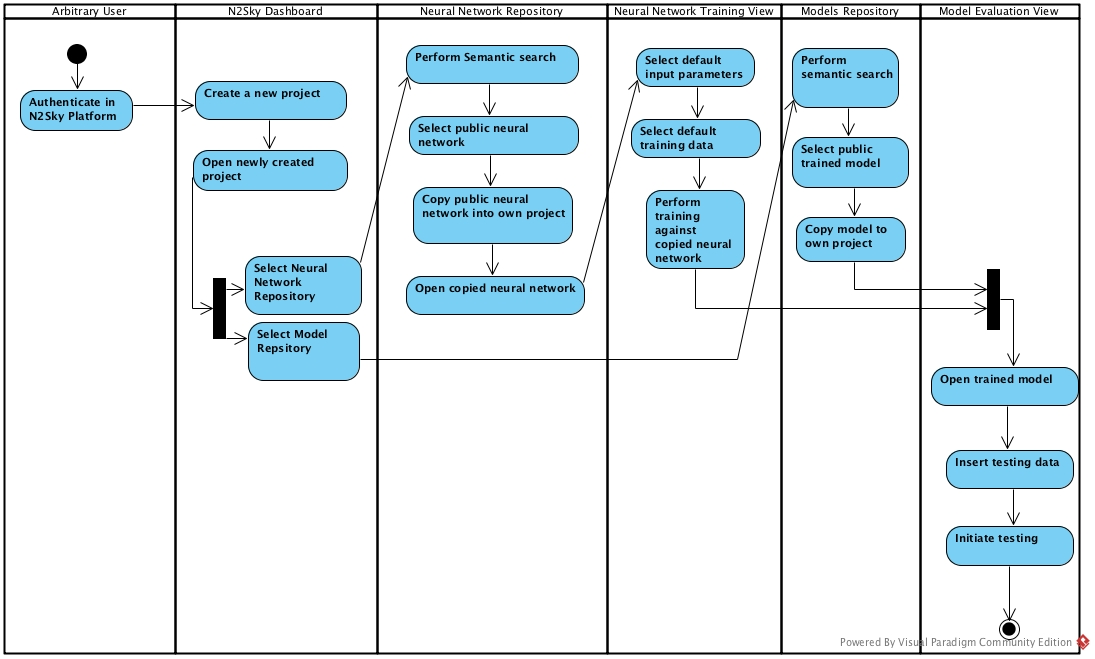
\includegraphics[width=\linewidth]{components/tutorial/img/training_arbitrary.jpg}
  \caption{Tutorial. Activity Diagram of using Network and Model Repositories}
  \label{fig:training_arbitrary}
\end{center}
\end{figure} 

\subsection{Creation of the neural network from the existing paradigm}\label{Creation of the neural network from the existing paradigm}

This case is related to neural network engineer user. 

\begin{figure}[htbp]
\begin{center}
  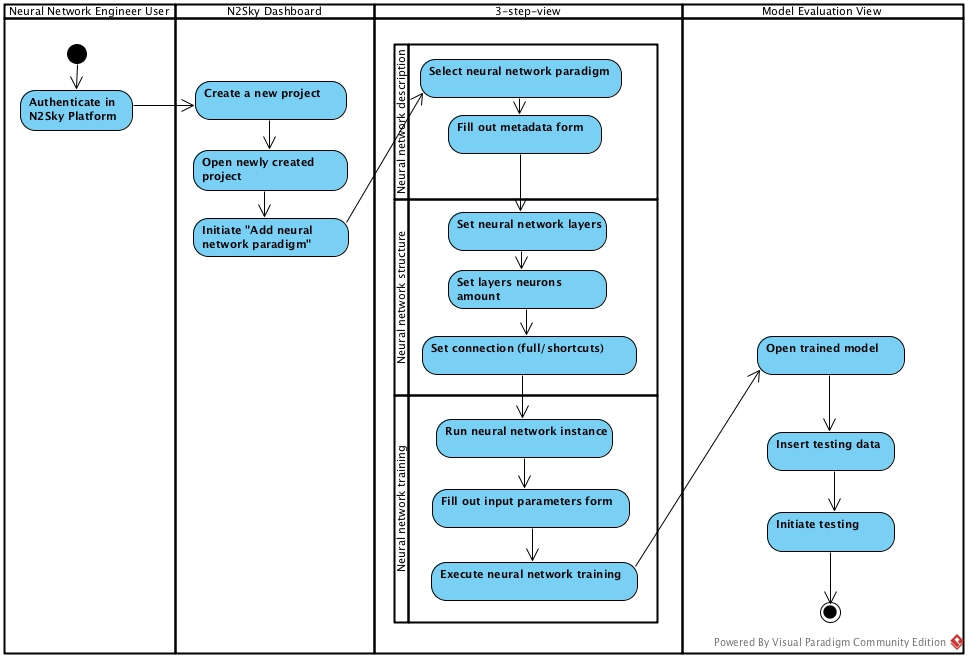
\includegraphics[width=\linewidth]{components/tutorial/img/tutorial_engeneer.jpg}
  \caption{Tutorial. Activity Diagram of creation the neural network from the existing paradigm}
  \label{fig:tutorial_engeneer}
\end{center}
\end{figure} 

\subsection{Upload own neural network paradigm}\label{Upload own neural network paradigm}


\begin{figure}[htbp]
\begin{center}
  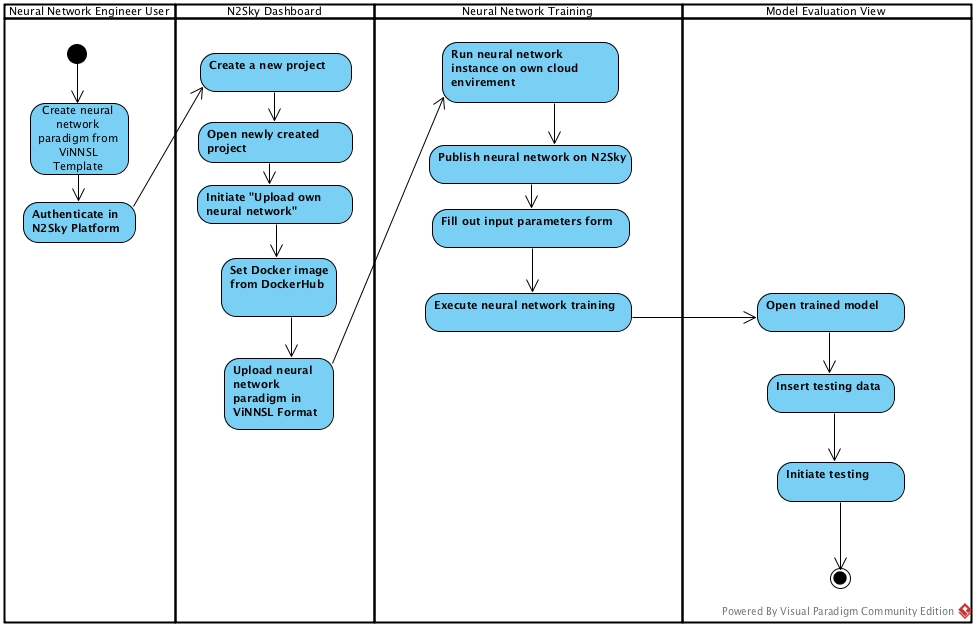
\includegraphics[width=\linewidth]{components/tutorial/img/tutorial_contribut.jpg}
  \caption{Tutorial. Activity Diagram of upload own neural network paradigm}
  \label{fig:tutorial_contribut}
\end{center}
\end{figure} 